\chapter{Cahier des charges}
\section{Objectifs}
Dans un premier temps nous voulons mettre en place un cloud privé sous la forme d'une IaaS avec OpenStack. L'objectif serait de permettre à des utilisateurs (des élèves par exemple) de créer des machines virtuelles très rapidement même sur des machines disposant de peu de ressources.\\

Ensuite nous voulons mettre en place une solution pour automatiser la configuration des instances. L'objectif serait de permettre à un/des administrateur(s) de modifier une configuration ou de rajouter une application même après qu'une image ait été créé.

\section{Fonctionnalités à implémenter}
\begin{itemize}
\item Un noeud de virtualisation avec KVM
\item Authentification \& Autorisations avec un LDAP
\item Interface simple d'utilisation pour la création d'images
\item Personnalisation des instances au lancement suivant l'utilisateur (montage des disques, ...)
\end{itemize}

\section{Perspectives}
\begin{itemize}
\item Haute-disponibilité, tolérance de pannes
\item Monitoring des machines physiques
\item Nœuds de virtualisations supplémentaires avec Xen, LXC, voir Hyper-V
\item Migration automatique des VMs après la chute d'un noeud
\end{itemize}
\chapter{Tâches}
\section{Tableau}
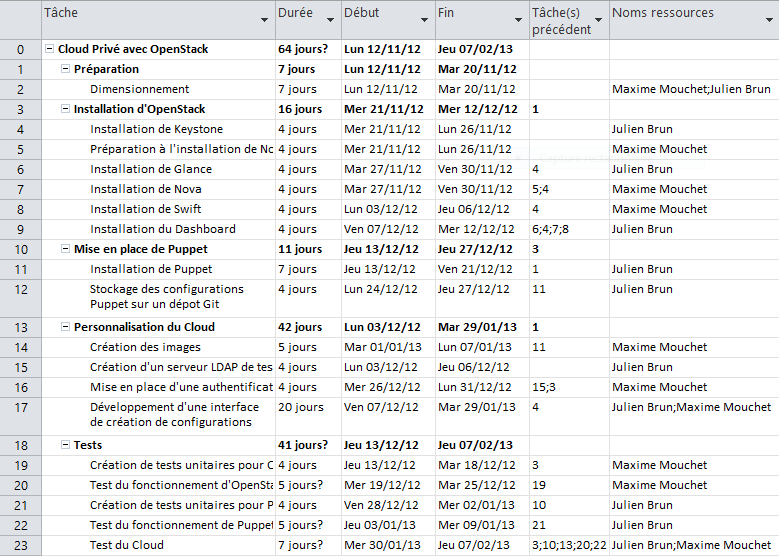
\includegraphics[width=19cm,angle=90]{images/liste.png}

\section{Liste détailée}
\subsection*{Tâche 2 : Dimensionnement}
\begin{description}
\item[Objectif :] Définir le matériel (nombre de machines) nécessaires
\item[Durée :]  1 semaine
\item[Assignée à :] Maxime Mouchet, Julien Brun
\end{description}

\subsection*{Tâche 4 : Installation de Keystone}
\begin{description}
\item[Objectif :] Installer et configurer le service de gestion d'identité et de l'API
\item[Durée :]  4 jours
\item[Assignée à :] Julien Brun
\end{description}

\subsection*{Tâche 5 : Préparation à l'installation de Nova}
\begin{description}
\item[Objectif :] Installer et configurer un système de virtualisation
\item[Durée :]  4 jours
\item[Assignée à :] Maxime Mouchet
\end{description}

\subsection*{Tâche 6 : Installation de Glance}
\begin{description}
\item[Objectif :] Installer et configurer le service de gestion des images
\item[Durée :]  4 jours
\item[Assignée à :] Julien Brun
\end{description}

\subsection*{Tâche 7 : Installation de Nova}
\begin{description}
\item[Objectif :] Installer et configurer le service de gestion des machines virtuelles
\item[Durée :]  4 jours
\item[Assignée à :] Maxime Mouchet
\end{description}

\subsection*{Tâche 8 : Installation de Swift}
\begin{description}
\item[Objectif :] Installer et configurer le service de stockage objet
\item[Durée :]  4 jours
\item[Assignée à :] Maxime Mouchet
\end{description}

\subsection*{Tâche 9 : Installation du Dashboard}
\begin{description}
\item[Objectif :] Installer et configurer l'interface web de gestion
\item[Durée :]  4 jours
\item[Assignée à :] Julien Brun
\end{description}

\subsection*{Tâche 11 : Installation de Puppet}
\begin{description}
\item[Objectif :] Installation de puppet master sur une machine et installation manuelle du client sur quelques instances virtuelles
\item[Durée :]  1 semaine
\item[Assignée à :] Julien Brun
\end{description}

\subsection*{Tâche 12 : Stockage des configurations Puppet sur un dépot Git}
\begin{description}
\item[Objectif :] Création d’un serveur Git, centralisation des fichiers de configurations
\item[Durée :]  4 jours
\item[Assignée à :] Julien Brun
\end{description}

\subsection*{Tâche 14 : Création des images}
\begin{description}
\item[Objectif :] Créer les images de machines virtuelles
\item[Durée :]  5 jours
\item[Assignée à :] Maxime Mouchet
\end{description}

\subsection*{Tâche 15 : Création d'un serveur LDAP de test}
\begin{description}
\item[Objectif :] Créer un serveur LDAP de test pour la tâche 16
\item[Durée :]  4 jours
\item[Assignée à :] Julien Brun
\end{description}

\subsection*{Tâche 16 : Mise en place d'une authentification via le LDAP}
\begin{description}
\item[Objectif :] Configurer Keystone pour utiliser un LDAP
\item[Durée :]  4 jours
\item[Assignée à :] Maxime Mouchet
\end{description}

\subsection*{Tâche 17 : Développement d'une interface de création de configurations}
\begin{description}
\item[Objectif :] Recherche d'une solution libre pour la création de fichiers de configurations. Sinon nous la développerons.
\item[Durée :]  20 jours
\item[Assignée à :] Julien Brun, Maxime Mouchet
\end{description}

\subsection*{Tâche 19 : Création de tests unitaires pour OpenStack}
\begin{description}
\item[Objectif :] Créer des tests automatisés pour OpenStack
\item[Durée :]  4 jours
\item[Assignée à :] Maxime Mouchet
\end{description}

\subsection*{Tâche 20 : Test du fonctionnement d'OpenStack}
\begin{description}
\item[Objectif :] Lancements des tests pour OpenStack et correction des problèmes si nécessaires
\item[Durée :]  5 jours?
\item[Assignée à :] Maxime Mouchet
\end{description}

\subsection*{Tâche 21 : Création de tests unitaires pour Puppet}
\begin{description}
\item[Objectif :] Crée des tests automatisées pour vérifier le bon fonctionement de Puppet
\item[Durée :]  5 jours?
\item[Assignée à :] Julien Brun
\end{description}

\subsection*{Tâche 22 : Test du fonctionnement de Puppet}
\begin{description}
\item[Objectif :] Lancements des tests pour Puppet et correction des problèmes si nécessaires
\item[Durée :] 5 jours?
\item[Assignée à :] Julien Brun
\end{description}

\subsection*{Tâche 23 : Test du Cloud}
\begin{description}
\item[Objectif :] Test global du système
\item[Durée :] 7 jours?
\item[Assignée à :] Julien Brun; Maxime Mouchet
\end{description}